\documentclass{llncs}

% A. Objectives
%    1. You should apply one of the techniques studied in the course to
%       solve this problem.
%    2. Devise and perform an empirical evaluation of your system.
%    3. Report your work.
%    4. All your documentation and source code should be available on your GitLab
%       project repository, as well as tasks and milestones. This will be part of
%       the evaluation.
%
% B. Deliverables
%    1. Progress report (by the end of May) describing
%     - selected approach and
%     - general project work plan
%     - group presentation of the report
%    2. Project report
%     - description of the problem
%     - updated material from the progress report
%     - description of your approach
%     - description of the software: installation, requirements and usage notes
%     - empirical evaluation
%    3. Software
%     - application and required libraries/software
%     - brief installation notes (README file)
%    4. Final Presentation
%     - description of your approach
%     - strengths and weaknesses
%     - empirical evaluation
%     - contribution of team members
%
% C. Timeline
%    1. 2018-05-30 Progress report and presentation
%    2. 2018-06-18 Software deliverable and final report
%    3. 2018-06-22 Final Presentation and Demo

\usepackage[utf8]{inputenc}
\usepackage[T1]{fontenc}

\usepackage{geometry}
\geometry{
  a4paper,
  textwidth=13cm,  % llncs has 12.2cm
  textheight=22cm, % llncs has 19.3cm
  heightrounded,
  hratio=1:1,
  vratio=2:3,
}

\usepackage[english]{babel}

\usepackage{hyperref}
\usepackage{bookmark}
\usepackage{csquotes}
\usepackage{multicol}
\usepackage{rotating}

\bibliographystyle{splncs03}

% In the appendix:
%\usepackage{longtable}
\usepackage{booktabs}

\setlength{\tabcolsep}{10 pt}

\usepackage{tikz,comment}
\usetikzlibrary{shapes.multipart,shapes.geometric,positioning,backgrounds,fit,calc,arrows.meta}

\pagestyle{plain}

\setlength{\columnseprule}{0.2pt}

\newcommand{\htw}{\emph{Hunt the Wumpus }}

\title{Hakuna Matata: A Logic-Based Agent for the \htw Game}
\subtitle{Project Report}
\author{Team White\\[2mm]Filippo~De~Bortoli \and Aneta~Koleva \and Lorenz~Leutgeb}
\institute{Free University of Bozen-Bolzano\\[3mm] \texttt{\{\href{mailto:filippo.debortoli@stud-inf.unibz.it}{filippo.debortoli},\href{mailto:aneta.koleva@stud-inf.unibz.it}{aneta.koleva},\href{mailto:lorenz.leutgeb@stud-inf.unibz.it}{lorenz.leutgeb}\}\newline @stud-inf.unibz.it}}

\begin{document}

\maketitle
\thispagestyle{plain}

\begin{abstract}
  The assigned task is to develop an intelligent agent that plays the \htw game, by using a logic-based approach in its implementation.
  In order to complete a run of the game, this agent has to be able to face several challenges, like the incompleteness of the available information about the state of the world or the search for the best strategy to employ.
  The chosen approach is to develop a hybrid agent that relies on an ASP core to actuate its strategy and on graph-theory techniques to obtain additional insights on how to proceed in the exploration of a dungeon.
  To assess the performance of our agent, we implemented an omniscient agent that obtains an optimal score for a given dungeon and we ranked our agent against it.
  In this report, we introduce our solution to this task, by detailing the architecture of the agent and describing the chosen strategy, the heuristics and the obtained results.
\end{abstract}

\section{Problem Statement}
%TODO Define what \htw is, all its rules and constraints.
%TODO Mention that it is also an example in the standard textbook AIMA and thus suited as an exercise in logic-based AI.

\htw is a single player computer game, first released in 1975.
It is best known as a toy-problem in the field of Artificial Intelligence and has been thoroughly analysed by Russell and Norvig in~\cite{book:aima}, where it has been used to introduce the reader to a logic-based approach to \emph{Knowledge Representation} (KR). 

The game is played in the wumpus world(a cave) which is represented as a grid (default size 4x4) and in this world there are few challenges for the player. Each cell on the grid is a room which is connected by passageways with its orthogonally adjacent cell and in one of these cells there is wumpus, a beast that eats the player if he enters the room. The player has only one arrow, that's one opportunity for shooting the wumpus. In addition, some of the rooms are bottomless pits and if the player wanders in these rooms it will stay trapped. The main goal of the player is while facing these challenges, to find the hidden gold and leave the cave alive. At the beginning of the game, the player is always positioned on cell [1,1], facing to the right and has 0 points. From here it can use three moves : \emph{Forward}, \emph{TurnLeft}, \emph{TurnRight} for discovering its environment and three actions \emph{Shoot}, \emph{Grab} and \emph{Climb} for shooting the arrow, grabbing the gold and climbing out of the cave respectively. For each of the moves and actions the player loses 1 point and 10 points when using the arrow. When eaten by the wumpus or trapped in pit, loses 1000 points, and for climbing out of the cave with the gold gains 1000 points. Whenever the player goes to a new cell, it has five sensors that give information about:
\begin{description}
	\item[Stench]{whether the Wumpus is in adjacent cell}
	\item[Breeze]{whether there is a pit in adjacent cell}
	\item[Glitter]{when the gold is in the current cell}
	\item[Bump]{whether the player has hit a border}
	\item[Scream]{whether the Wumpus is hit by the arrow}
\end{description}
The locations of the gold and the wumpus are chosen randomly with uniform distribution in each cell other then the start. Additionally each cell can be a pit with probability 0.2.

In~\cite{book:aima}, the environment which represents the Wumpus World is is described as discrete, static, single-agent and partly-observable. For an agent in such environment the main challenge is its initial ignorance of the configuration of the world and using logical reasoning can be helpful for solving this. 

\section{Approach}

In this section, we describe the ideas and the concepts that underlie our approach to the assigned task.
In particular, we single out those aspects that are relevant to the understanding of the behaviour that the Hakuna agent shows during a run of the game.

For the purpose of this project, we decided to implement a logic-based agent, that plays \htw employing both Answer Set Programming (ASP, in~\cite{ASPprimer} a detailed introduction is given) and suitable search techniques --- borrowed from graph theory --- to explore the search space and find an optimal strategy to finish the game with the maximum score.

\subsection{ASP and World Knowledge}

The environment in which the agent is playing is \emph{discrete} and \emph{static}, since the wumpus, the gold and the pits do not move throughout the dungeon.
Therefore, the knowledge inferred by the agent at each point in time can be accumulated to circumscribe the search space in further moments in time.
Initially, the agent's \emph{knowledge base} (KB) is populated with basic geometric knowledge (e.g. relation between directions), what is percepted in its initial position and what are the known world sizes.

\paragraph{Incomplete knowledge.} One of the challenges of \htw is that a non-omniscient player starts the game with an incomplete knowledge of the world.
By exploring the dungeon and perceiving what is in each new explored room, an agent can obtain additional insights about the state of the world and reshape its strategy according to it.
As we want to be able to model non-monotonic reasoning --- if a room, previously thought to contain a pit, turns out to be safe, the agent should be able to infer this --- and to generalise statements by writing non-ground schematas, our system of choice is Answer Set Programming, which allows to model the problem in a logic fashion and achieves non-monotonic reasoning through \emph{closed-world assumption} (CWA).
% TODO: explicitly refer to SAT and SMT.
In particular, the DLV solver~\cite{DLV-system} has been embedded in the architecture of the agent, to be called at every point in time to infer the additional knowledge obtained by the agent, after grounding its KB.
This approach allows the agent to correctly derive what is logically right from it's knowledge base. Moreover DLV is able to process incomplete knowledge which the agent has while overcoming its initial ignorance with logical reasoning.

\paragraph{Safety.} As the Hakuna agents tries to maximise its score by minimising its death chances, the need of a concept of \emph{safety} arises.
Namely, the agent moves towards some room if it is not aware of any danger lying in it (this is an application example of CWA) and marks as certainly \emph{safe} each room that he enters without dying.
This, together with the other perceived information, allows the agent to ``draw'' an internal representation of the world that will progressively allow it to move further or search for alternative exploratory routes.

\paragraph{Size of the world.} The agent proceeds by assuming that the world has a certain size, initially set to $1 \times 1$.
Every time the agent succeeds to move to a room which coordinates exceed the assumed size of the world, for example $N \times N$, the KB is updated to assume that the world has size $N+1 \times N+1$.
Otherwise, if a \emph{bump} is percepted, it infers the real size of the world and this will not be modified afterwards.

\paragraph{Unsafety.} The agent's policy for unsafe situations is the following:
\begin{itemize}
	\item If a room signalling a nearby unsafe room is entered, turn backwards and explore the next \emph{safe} and unexplored room. A signal can be a perceived \emph{stench} or a \emph{breeze}.
	\item If the location of two stenches lying on a same axis is known, the wumpus is evinced to lie between them.
	\item If the location of two stenches lying on a same diagonal is known and one of the common neighbours is known to be safe, the other neighbouring room is inferred to contain the wumpus.
	\item If a breeze is found, all the unexplored neighbours are marked as rooms possibly containing a pit.
	\item If a room without breezes is found nearby one marked as a possible pit, the KB is updated to state that such a room is instead not containing any pit. 
\end{itemize}

% maybe mention that we can write strong constraints, not sure if still have that

\subsection{Agent Modes and Strategies}

In order to simplify the implementation of the agent and the way it choses its next action we introduce four different modes of playing in which the agent can be at any time. This helps to abstract and in different modes enable and disable different possible actions. It also made it easier for developing the code. 
While playing, our agent can be in exactly one from four available modes.

\paragraph{Explore} The agent is in this mode until it discovers the gold or there are more cells which should be explored. These are cells which are known to be reachable, safe and not yet explored. 

\paragraph{Grab} Once the agent is in the cell where can perceive glitter, its next action is to grab the gold and in this moment is in mode \emph{grab}. 

\paragraph{Kill} In order for the agent to deduce that is in mode \emph{kill} few conditions need to be satisfied. First it should not be in mode grab or explore and the gold is still not grabbed. Next it should be able to attack the wumpus. A necessary precondition for attacking the wumpus is to deduce that it can try to kill and it should try to do so. Can try to kill the wumpus only if it's on a safe cell, it perceives stench and it's with orientation facing the cell where the wumpus possibly is. 
Should try to kill can be derived if it's known that it can try to kill the wumpus and none of the preconditions for don't shoot are known to be true. These preconditions for not shooting include: the arrow is not available, the wumpus is in a cell with a pit, the wumpus is already dead and the gold is already grabbed. 
% TODO: add something about killing to explore.

\paragraph{Escape} The last available mode is \emph{escape}, in which the agent is if it's not in any of the other three modes. The agent is in this mode after grabbing the gold or after not being able to explore any other cells and leaves the cave empty handed.

\subsection{$A^{\star}$ Search and World Exploration}

As a way to exploit the partial knowledge of the world and improve the subsequent planning, the agent builds an internal representation of a reachability graph.
The vertexes of such a graph represent those configuration lying in the \emph{frontier} of the agent, that is, safe and reachable rooms that are yet to be explored.
The edges of the graph represent the reachability of a configuration from another.
The edges are weighted according to the following cost function: given the actual configuration $C = (X,Y,O)$ and a target configuration $C^\prime = (X^\prime,Y^\prime,O^\prime)$,
$$
	g(C,C^\prime) := M((X,Y),(X^\prime,Y^\prime)) + R((X,Y),O,(X^\prime,Y^\prime))
$$
where $M$ represents the \emph{Manhattan distance}~\cite{Manhattan} between the two rooms and $R$ is the least number of turns needed by the agent to reach $(X^\prime,Y^\prime)$ from $(X,Y)$.
% For better exploration of the world, we build a graph that represents reachability (with cost) for all cells. Then we use \emph{Manhattan distance}~\cite{Manhattan} as a cost function for calculating the cost for moving from a cell to a cell. We also consider the rotation cost  when the agent reasons about the number of moves it needs to make in order to move from a cell to another cell. To calculate this cost, first the cost of all turns on the way from current cell to a destination cell is calculated and to this is added the cost of departing the current cell (whether the agent needs to turn before leaving).
To compute the minimal cost needed to reach the target room the agent performs an \emph{$A^{\star}$ search} (as first introduced in~\cite{AStar}).%s : \(f(n) = g(n) + h(n)\). \
In order to efficiently use this algorithm next and goal cell must be known. 
First the goal cell is calculated and based on this result, the next cell is decided.  The choice of a goal cell depends on the current mode of the agent. If it's in mode \emph{explore}, goal is a reachable cell which is safe and hasn't been explored yet. If the agent's mode is \emph{kill}, then the goal is a cell which is safe and from which the wumpus can be shot.
In our program \(g(n)\) represents the cost of the path from the current cell to the next cell \(n\), and \(h(n)\) represents the heuristic estimated cost of the cheapest path from cell \(n\) to the goal cell. 

%TODO How does our agent explore the world (A*-search)
%not sure if here should be explained the purpose of pathTurnCost,
%departureTurnCost and rotCost or leave that for implementation
% @filippo-23:20 28/05/2018: I think that details can be left for Implementation, but if they are used to define cost/heuristic, I would briefly mention them here. 

\begin{figure}
	\begin{center}
		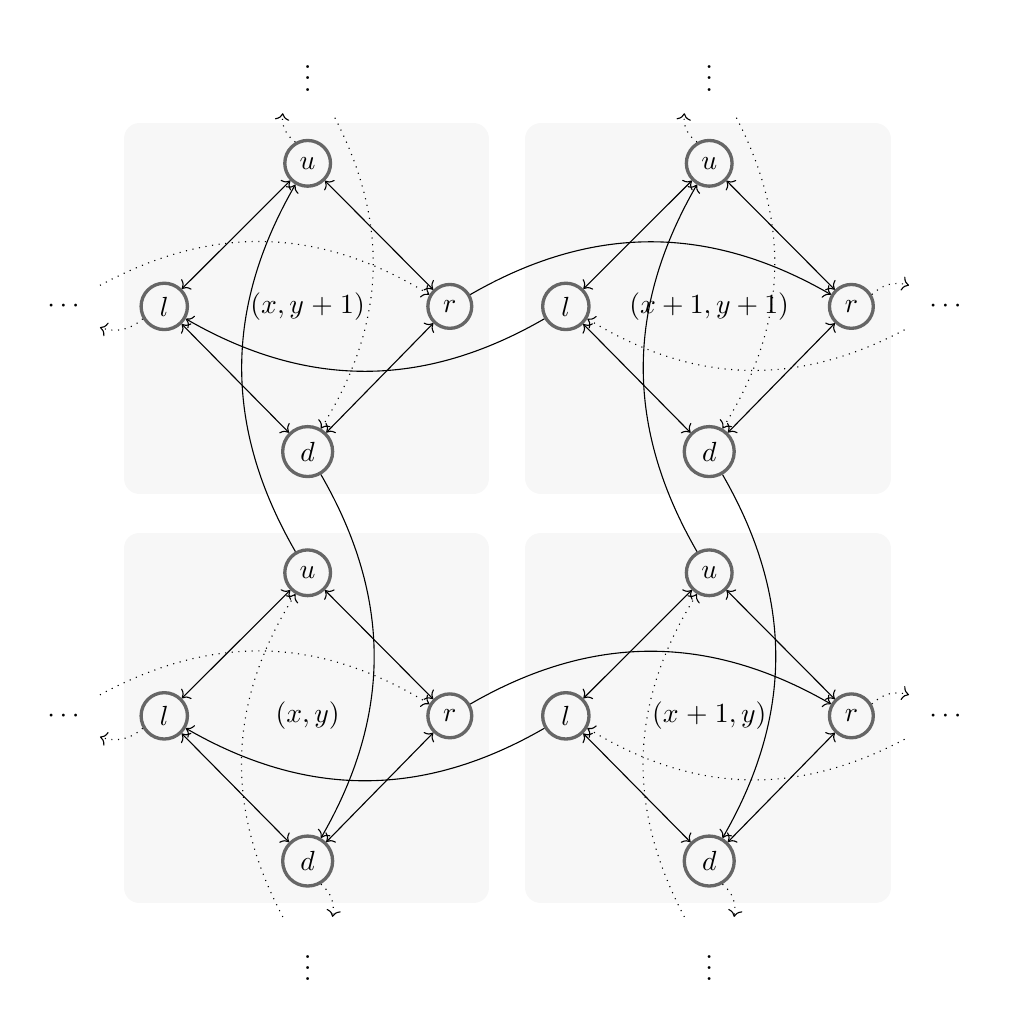
\begin{tikzpicture}[roundnode/.style={circle, draw=black!60, very thick,minimum size=4mm}]
	\begin{scope}
		\node[regular polygon, regular polygon sides=4, align=center, text width={width("$(x + 1, y + 1)$")}] (n11) {$(x, y)$};
		\node[roundnode] (u11) [above=-1mm of n11] {$u$};
		\node[roundnode] (l11) [left=-1mm of n11] {$l$};
		\node[roundnode] (r11) [right=-1mm of n11] {$r$};
		\node[roundnode] (d11) [below=-1mm of n11] {$d$};
		\draw [<->] (u11) -> (l11);
		\draw [<->] (u11) -> (r11);
		\draw [<->] (d11) -> (l11);
		\draw [<->] (d11) -> (r11);
	\end{scope}
		
	\begin{scope}[xshift=5.1cm]
		\node[regular polygon, regular polygon sides=4, align=center, text width={width("$(x + 1, y + 1)$")}] (n21) {$(x + 1, y)$};
		\node[roundnode] (u21) [above=-1mm of n21] {$u$};
		\node[roundnode] (l21) [left=-1mm of n21] {$l$};
		\node[roundnode] (r21) [right=-1mm of n21] {$r$};
		\node[roundnode] (d21) [below=-1mm of n21] {$d$};
		\draw [<->] (u21) -> (l21);
		\draw [<->] (u21) -> (r21);
		\draw [<->] (d21) -> (l21);
		\draw [<->] (d21) -> (r21);
	\end{scope}
		
	\begin{scope}[yshift=5.2cm]
		\node[regular polygon, regular polygon sides=4, align=center, text width={width("$(x + 1, y + 1)$")}] (n12) {$(x, y + 1)$};
		\node[roundnode] (u12) [above=-1mm of n12] {$u$};
		\node[roundnode] (l12) [left=-1mm of n12] {$l$};
		\node[roundnode] (r12) [right=-1mm of n12] {$r$};
		\node[roundnode] (d12) [below=-1mm of n12] {$d$};
		\draw [<->] (u12) -> (l12);
		\draw [<->] (u12) -> (r12);
		\draw [<->] (d12) -> (l12);
		\draw [<->] (d12) -> (r12);
	\end{scope}
		
	\begin{scope}[yshift=5.2cm,xshift=5.1cm]
		\node[regular polygon, regular polygon sides=4, align=center] (n22) {$(x + 1, y + 1)$};
		\node[roundnode] (u22) [above=-1mm of n22] {$u$};
		\node[roundnode] (l22) [left=-1mm of n22] {$l$};
		\node[roundnode] (r22) [right=-1mm of n22] {$r$};
		\node[roundnode] (d22) [below=-1mm of n22] {$d$};
		\draw [<->] (u22) -> (l22);
		\draw [<->] (u22) -> (r22);
		\draw [<->] (d22) -> (l22);
		\draw [<->] (d22) -> (r22);
	\end{scope}
		
	\begin{scope}[xshift=8.1cm]
		\node[regular polygon, regular polygon sides=4] (n31) {$\cdots$};
	\end{scope}
		
	\begin{scope}[yshift=5.2cm,xshift=8.1cm]
		\node[regular polygon, regular polygon sides=4] (n32) {$\cdots$};
	\end{scope}

	\begin{scope}[yshift=8.2cm]
		\node[regular polygon, regular polygon sides=4] (n13) {$\vdots$};
	\end{scope}

	\begin{scope}[yshift=8.2cm,xshift=5.1cm]
		\node[regular polygon, regular polygon sides=4] (n23) {$\vdots$};
	\end{scope}

	\begin{scope}[xshift=-3.1cm]
		\node[regular polygon, regular polygon sides=4] (n01) {$\cdots$};
	\end{scope}

	\begin{scope}[yshift=-3.1cm,xshift=5.1cm]
		\node[regular polygon, regular polygon sides=4] (n20) {$\vdots$};
	\end{scope}

	\begin{scope}[yshift=-3.1cm]
		\node[regular polygon, regular polygon sides=4] (n10) {$\vdots$};
	\end{scope}

	\begin{scope}[yshift=5.2cm,xshift=-3.1cm]
		\node[regular polygon, regular polygon sides=4] (n02) {$\cdots$};
	\end{scope}

	\path [->] (r11) edge [bend left] (r21);
	\path [->] (l21) edge [bend left] (l11);
	\path [->] (u11) edge [bend left] (u12);
	\path [->] (d12) edge [bend left] (d11);
	\path [->] (u21) edge [bend left] (u22);
	\path [->] (d22) edge [bend left] (d21);
	\path [->] (r12) edge [bend left] (r22);
	\path [->] (l22) edge [bend left] (l12);

	\path [->, dotted] (r21) edge [bend left] (n31);
	\path [->, dotted] (r22) edge [bend left] (n32);
	\path [->, dotted] (u12) edge [bend left] (n13);
	\path [->, dotted] (u22) edge [bend left] (n23);
	\path [->, dotted] (l11) edge [bend left] (n01);
	\path [->, dotted] (d11) edge [bend left] (n10);
	\path [->, dotted] (l12) edge [bend left] (n02);
	\path [->, dotted] (d21) edge [bend left] (n20);

	\path [<-, dotted] (l21) edge [bend right] (n31);
	\path [<-, dotted] (l22) edge [bend right] (n32);
	\path [<-, dotted] (d12) edge [bend right] (n13);
	\path [<-, dotted] (d22) edge [bend right] (n23);
	\path [<-, dotted] (r11) edge [bend right] (n01);
	\path [<-, dotted] (u11) edge [bend right] (n10);
	\path [<-, dotted] (r12) edge [bend right] (n02);
	\path [<-, dotted] (u21) edge [bend right] (n20);

	\begin{pgfonlayer}{background}
		\filldraw[line width=4mm,join=round,black!3]
			(u11.north -| r11.east) rectangle (d11.south -| l11.west)
			(u21.north -| r21.east) rectangle (d21.south -| l21.west)
			(u12.north -| r12.east) rectangle (d12.south -| l12.west)
			(u22.north -| r22.east) rectangle (d22.south -| l22.west)
		;
	\end{pgfonlayer}
\end{tikzpicture}

	\end{center}
	\caption[Cost Calculation and Reachability graph]{Cost Calculation and Reachability graph for a grid of four rooms. Here $u$ (up), $d$ (down), $l$ (left), and $r$ (right) naturally correspond to orientations, while a cluster of four nodes corresponds to a room. Note that straight edges represent turns and bent edges represent going forward.}
	\label{fig:graph}
\end{figure}

\subsection{Reasoning modes and Planning}

One feature of our ASP encoding of the playing agent is that a unique stable model is generated from it, for each call of the DLV solver.
This is due to design choices: Hakuna is encoded in such a way that, at each point in time, a unique goal and a unique next step can be inferred.
To achieve this, tie-breaking constraints and rules have been introduced.
As a side effect, the cautious and the brave consequences that can be drawn from the ASP program are the same.
By lifting some of these constraints, the uniqueness of the stable model would get lost and cautious reasoning might bring to different conclusions.
Such a feature could be exploited to introduce a form of ``don't know'' non-deterministic choice for the agent, in planning its next moves and goals.
If not properly handled, though, this might lead to a loss of some desired properties of our agent, for example, the minimization of the costs in the \emph{explore} mode.

\subsection{Taking Risks}
Equipped with above notion of safety, the agent is able to navigate the network of rooms without failing. However, in some scenarios, this implies that the gold is not found, e.g.\ because it is obstructed by the perception of breezes, even though it could be reached. We generously call the action of going forward into a cell that might contain a pit or the wumpus \emph{taking a risk}. The connection to incomplete knowledge about the game is apparent, i.e.\ in a game with perfect knowledge, there are no risks of this character, since the outcome of every action is certain.

In early phases of designing our approach, we also considered how risk taking fits in. We investigated into approaches that may yield a quantification and finally a probabilistic decision procedure for the agent. However our conclusion is that necessary theoretic foundations like Markov processes and Bayesian models (or possibly others, unknown to us) would mean departing from a logic based agent.

%To reason about risk taking, we compare the best possible outcome and the worst possible one. For the sake of simplicity we only consider theOf utmost importance for these considerations is how failure of the agent is scored, and how probable that failure is. The world simulator that we worked with defines a probability of 20\% for any room (except the initial room) to contain a pit or the wumpus, and a score of -1000 pts.\ in this case the agent enters such a room.  Intuitively, risk taking should therefore have at least an average utility of 1000 pts.\ in order to break even for growing sample sizes. We argue that reaching this utility is impossible: Given that the agent is able to safely return to its initial position afterwards, the action with the highest utility is grabbing the gold (999 pts., 1000 for leaving the cave with the gold, and -1 pt.\ for grabbing it). Thus, even if the gold happens to be in the same room that the agent enters as it is taking a risk,   Reaching this utility is impossible, since the action with the highest

\section{Implementation}
%TODO Short section where we describe the system, referring to the appendix (see below)
%TODO as well as that we used DLV.
%TODO Generate and include the Dependency Graph
%TODO Autopilot (if it works at some point)
%TODO Refer to usage file for actually running the system.
%TODO mention WSU.
%TODO mention ASP-Lite

In this section, we briefly describe how the agent described in the previous section was implemented. Note, however that for the implementation in its full detail we refer to Appendix \ref{hunt-the-wumpus}. Further, for the Python code that hosts the ASP based implementation and usage notes we refer to the project repository.

The Python host keeps state in memory as the game progresses. This includes perceptions for all visited rooms, from which room and in which orientation the agent has shot the arrow (if applicable), whether the wumpus is dead or alive, and whether the agent has ever performed the \emph{grab} action. All this information is considered the \emph{memory} of the agent, and encoded as facts every time the logic program is invoked for the purpose of reasoning about the next action.

\begin{figure}
\begin{center}

		
			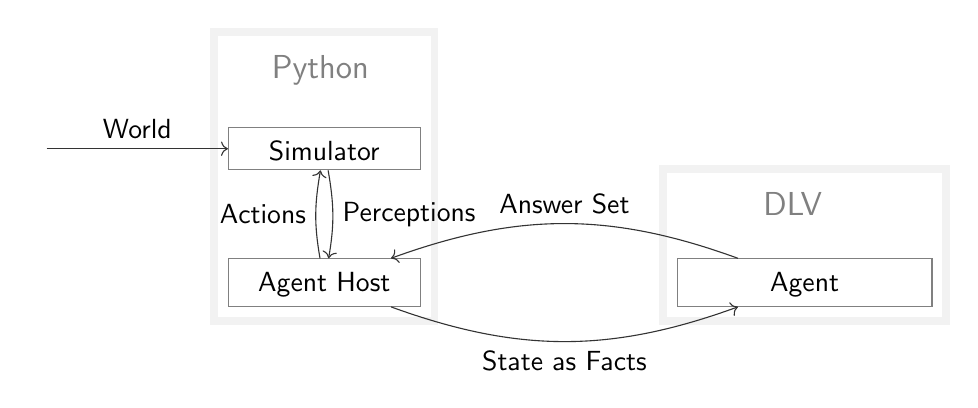
\begin{tikzpicture}[
			node distance=1cm and 5mm,
			every node/.style={font=\sffamily},
			title/.style={font=\color{black!50}\sffamily},
			typetag/.style={rectangle, draw=black!50, font=\sffamily, anchor=west, text height=3mm, align=center}
			]
			
			\node (lp) at (0, -1cm) {};
			\node (as) at (0, -3.2cm) {};
			
			\node (gl) at (3.6cm, 0) [align=center, text width=2.1cm, title] { \large Python };
			
			\node (par) [below=of gl.west, text width=22mm, typetag] { Simulator };
			\node (gro) [below=1.7cm of par.west, text width=22mm, typetag] { Agent Host };
			
			\node (g) [draw=gray!10, line width=1mm, inner sep=5pt, fit={(gl) (par) (gro)}] {};
			
			\node (sl) at (9.6cm, -1.7cm) [align=center, text width=2.7cm, title] { \large DLV };
			
			\node (ngs) [below=of sl.west, text width=3cm, typetag] { Agent };
			
			\node (s) [draw=gray!10, line width=1mm, inner sep=5pt, fit={(sl) (ngs)}] {};
			
			\draw [->, draw=black!80] (gro) to [out=340, in=200] node [midway, below] {State as Facts} (ngs);
			\draw [->, draw=black!80] (ngs) to [out=160, in=20] node [midway, above] {Answer Set} (gro);
			
			\draw [->, draw=black!80] (par) to [out=280, in=80] node [midway, right] {Perceptions} (gro);
			\draw [<-, draw=black!80] (par) to [out=260, in=100] node [midway, left] {Actions} (gro);
			
			\draw [->, draw=black!80] (lp) -- (par) node [midway, above] {World};
			\end{tikzpicture}
	
\end{center}
\caption{Architecture of the Implementation}
\label{fig:architecture}
\end{figure}

\subsection{Autopilot}

One optimization that was employed to decrease the overall run time of the agent in the course of a game is what we call the autopilot. In this section we motivate the reason for introducing this component and describe it and its interaction with the rest of the implementation briefly.

It is obvious that most of the run time is spent computing a stable model by the ASP solver, since both the world simulator as well as the Python host program do not solve hard computational problems. With this in mind, the motivation to call the ASP solver as rarely as possible is apparent. In particular, since the ASP program is deterministic, the resulting answer sets only change with new input.

Choice of the goal is influenced by past perceptions and the current location and orientation of the agent. However, as long as the goal is not reached, the ASP program will \enquote{steer} towards it: The cost to reach the goal gradually gets smaller, until finally it is reached. As long as no new room is explored, goal selection remains stable.

This mechanic is what we exploit with the autopilot. Once a goal is chosen, a path that leads there is planned and forwarded to the world simulator without invoking the solver. This setup requires careful selection rules for the goal and detection of unsafe rooms.

In order to prevent planning of paths that pass through unsafe rooms, all incoming edges to such rooms may be assigned an infinite cost, thus effectively making them unreachable.

% TODO Mentionhow we keep the search space for cost function small

% TODO Mention that we digressed into dependency graphs, alternate syntax
% TODO Mention bad/1 and why we introduced it instead of looking at an inconsistent program

%\begin{sidewaysfigure}[ht]
%\includegraphics[width=1\textwidth]{dep}
%\caption[Dependency Graph of the Logic Program]{Dependency Graph of the Logic Program. }
%\end{sidewaysfigure}

% \subsection{Autopilot}

% An enhancement that has been found to effectively impact the execution time of the agent is the introduction of an \emph{autopilot}.
% The autopilot is activated when the following requirements are met:
% \begin{itemize}
% 	\item The agent is either in \emph{explore} or \emph{escape} mode;
% 	\item No priorities are in place, that is, the agent is not trying to grab, shoot, aim or climb.
% \end{itemize}
% Given these conditions, the Python agent host takes control, performs an $A^{\star}$ search over the graph to find the best path to reach the next goal, by assigning an additional cost of $1$ to those rooms that are yet unknown to be safe.
% Then, the game will be executed without calling the ASP solver, as long as the selected goal has not been reached.
% Once the goal room has been reached, the Python host calls again the ASP solver, to infer the next move.

% This approach brings a relevant decrease in the execution time: indeed, every time the autopilot is activated, the execution cost required by the calls to DLV is saved.

\section{Evaluation}

In this section, we explain how the empirical evaluation of our agent has been carried out.
In particular, we describe which experiments our agent has been tested with, which parameters have been collected and how its performance has been assessed.
To produce a satisfying evaluation, we generated a testing suite and, in order to obtain a reliable reference, we built an omniscient agent.

\subsection{Testing Suite}

The implementation of the agent Hakuna has been continuously refined by testing it against a suite of dungeons.
The instances contained in the suite have been randomly generated using the Wumpus World Simulator~\cite{WWS} provided in the assignment.
This prevented the suite from containing building biases, like non-uniform distribution of the pits and non-overlapping entities in the dungeon.
Each entry of this suite, bundled together with our implementation of the agent, is characterized by the \emph{size} of the dungeon and the \emph{seed} used to generate it; this allows one to reproduce the creation of each dungeon collected in the suite.
In Table~\ref{tbl:test}, the composition of the testing suite is outlined.

\begin{table}[t]
	\label{tbl:test}
	\centering
	\begin{tabular}{rrrrr}
	\toprule
	\multicolumn{1}{c}{World size} & \multicolumn{1}{c}{instances} & \multicolumn{1}{c}{avg. gap} & \multicolumn{1}{c}{stddev gap} & \multicolumn{1}{c}{avg. wall-time (s)}\\
	\midrule
	4 & 160	& 419 & 488 & 0.1440 \\
	5 & 80  & 464 & 493 & 0.2656 \\
	6 & 80  & 634 & 474 & 0.4600 \\
	7 & 40  & 630 & 468 & 2.8005 \\
	8 & 40  & 653 & 471 & 3.8736 \\
	9 & 20  & 557 & 490 & 4.7723 \\
	10 & 20 & 714 & 452 & 11.3828 \\
	11 & 10 & 785 & 414 & 0.1573 \\
	12 & 10 & 595 & 498 & 0.5594 \\
	13 & 5  & 383 & 524 & 0.0158 \\
	14 & 5  & 600 & 506 & 11.8238 \\
	\bottomrule\\
	\end{tabular}
	\caption{Some aggregated results obtained by assessing Hakuna against our testing suite.}
\end{table}

Each world has been generated by taking into account the rules of \htw: indeed, each instance has a squared shape, it contains only one wumpus, one unit of gold and it may contain several pits, sparse through the dungeon.

\subsection{An omniscient agent}

In order to assess the performance of our Hakuna agent, we built another agent, whose score has then been referenced in evaluating our results.

The particularity of this other agent is \emph{omnisciency}: indeed, our assumption is that it has complete knowledge of the world, of the exact location of the unsafe cells and of the gold.
In this setting, the search for the optimal solution can be reduced to the computation of the shortest path from the initial point over an \emph{action graph} built in the following way:
\begin{itemize}
	\item Each node is a configuration $(X,Y,O)$ that the agent can assume.
	\item Two configurations are linked by an edge if one can be reached by the other.
	\item The weight of each edge is $1$ if the target is not a configuration in the same position as the Wumpus's, $10$ otherwise; this reflects the need to kill the Wumpus in order to pass through it.
\end{itemize}
A shortest path over this graph reflects the shortest path in the dungeon from a configuration to another.
Here, the cost function is the same that has been previously employed.

Then, the perfect agent behaves as follows: if the gold is unreachable, thus it lies in a pit, it immediately climbs; otherwise, he takes the shortest path to the cell containing the gold, grabs it and comes back to the initial position from the same path, to finally climb.

\subsection{Performance assessment}

For each instance, a run of the omniscient agent and one of the Hakuna agent have been recorded and their scores collected for comparison.
Being ours a pure logic-based approach, the score obtained by both agents on an instance can be exactly reproduced, given the agent and the instance; this would not be the case, if probabilistic reasoning was taken into account.
From the collected data, the gap between the results scored by the two agents in each instance has been computed, and the sample mean and standard deviation have been computed.

After data collection, we investigated those instances where the the perfect agent outperformed Hakuna, to understand the possible causes and search for plausible improvements.
What we have found out can be summarised as the following:
\begin{itemize}
	\item Hakuna performed similarly to the agent in those instances where the gold was reachable by just exploring the dungeon and in those where killing the Wumpus led to the discovery of a safe path to the gold.
	\item On the other hand, Hakuna was outperformed in those instances where the phenomenon of \emph{breeze walls} happened: the location of the breezes brought the agent to infer a disposition of possible pits that blocked its way to the gold, even though there were no pits between it and the reward.
	\item On instances where gold was unreachable, the agent lost on average a small amount of points before concluding that the search was useless and climbing back to the exit.
\end{itemize}

With increasing sizes, the gap between the score of the omniscient agent and the one obtained by Hakuna tends to increase: this might be caused by the greater amount of rooms that Hakuna has to visit, while it is in \emph{explore} mode. 

During the development stage, the execution time of the agent on each instance has been collected.
This allowed us to effectively evince that the introduction of the autopilot brought significant time savings in several instances, for example, the ones where most of the time was spent in exploring the dungeon.
The collected data are displayed in Table~\ref{tbl:test}. Information about mean execution time for samples drawn for dungeon size greater than 10 might be misleading, because of the small size of the samples.

\section{Conclusion}

% TODO Conclusion: implementing an agent is possible, we implemented an agent according to a logic based repr of the problem that exhibits a specific behaviour: is trying to stay alive (maximize score) and during the development phase we tested . the implementation merges several ideas and led to problems but we considered the advanteges and drawbacks of a logic based approach. leads to graph based solution. we managed to improve the performance of our agent by pruning the search space

\paragraph{Future Work}
% TODO we considered some approaches that go beyond logic and we are interested in a hybrid approach with probabalistic reasoning
% TODO Consider other variants of the game (multi agent, oracle, bats, other topologies not square grids)

\newpage
\newgeometry{
  left=1cm,  % llncs has 12.2cm
  right=1cm,
  top=1cm, % llncs has 19.3cm
  bottom=2cm,
}
\appendix
\footnotesize

\begin{multicols}{2}
\hypertarget{hunt-the-wumpus}{%
\section{Hunt the Wumpus}\label{hunt-the-wumpus}}

This is an implementation of an agent that plays ``Hunt the Wumpus''.

Input should be given as follows:

\begin{verbatim}
#maxint = 1000.
\end{verbatim}

\hypertarget{constants}{%
\subsection{Constants}\label{constants}}

We use constants to encode concrete orientations, actions and modes, and
one corresponding predicate to all of them respectively.

According to \texttt{wumpus.common.Orientation} we define orientations.

\begin{verbatim}
#const right = 0.
#const up    = 1.
#const left  = 2.
#const down  = 3.

isOrientation 0..3
\end{verbatim}

According to \texttt{wumpus.common.Action} we define actions.

\begin{verbatim}
#const goforward = 0.
#const turnleft  = 1.
#const turnright = 2.
#const grab      = 3.
#const shoot     = 4.
#const climb     = 5.

isAction 0..5
\end{verbatim}

According to \texttt{wumpus.agent.Mode} we define modes.

\begin{verbatim}
#const explore = 0.
#const escape  = 1.
#const kill    = 2.

isMode 0..3
\end{verbatim}

Additionally we designate two orthogonal orientations as axes.

\begin{verbatim}
axis right
axis up
\end{verbatim}

Being able to mirror orientations/turns will come in handy.

\begin{verbatim}
mirror         left right
mirror         up   down
mirror         O2   O1
        mirror O1   O2
\end{verbatim}

\hypertarget{world-size}{%
\subsection{World Size}\label{world-size}}

If the agent never bumped against a wall, it has no information about
the size of the world.

\begin{verbatim}
sizeKnown
        bump _ _
\end{verbatim}

We will therefore derive the size of the world from something already
known.

\begin{verbatim}
exploredSize     X
        explored X Y

exploredSize       Y
        explored X Y
\end{verbatim}

Since any cell we already explored certainly is part of the world, we
can use this information and guess that the world is ``just a little''
bigger than we already know.

\begin{verbatim}
size                            S
        not sizeKnown
        #succ             Sm    S
        #max              Sm Se
                exploredSize Se
\end{verbatim}

Of course, if the agent bumped, the size can be directly inferred.

\begin{verbatim}
size               S
        bump  Sm Y
        >     Sm Y
        #prec Sm   S

size               S
        bump  X Sm
        <=    X Sm
        #prec   Sm S
\end{verbatim}

\hypertarget{cells-neighbors-facing-and-bumps}{%
\subsection{Cells, Neighbors, Facing And
Bumps}\label{cells-neighbors-facing-and-bumps}}

Span the space of cells.

\begin{verbatim}
cell         X Y
        #int X
        #int   Y
        >      Y 0
        >    X   0
        <=     Y S
        <=   X   S
        size     S

corner 1 1

corner       X 1
        cell X 1
        size X
        sizeKnown

corner       1 Y
        cell 1 Y
        size   Y
        sizeKnown

corner       S S
        cell S S
        size S
        sizeKnown
\end{verbatim}

Two cells are different if any of the components X, Y are unequal.

\begin{verbatim}
diff         X1 Y1 X2 Y2
        cell X1 Y1
        cell       X2 Y2
        !=   X1    X2

diff         X1 Y1 X2 Y2
        cell X1 Y1
        cell       X2 Y2
        !=      Y1    Y2
\end{verbatim}

\hypertarget{distances-and-costs}{%
\subsubsection{Distances and Costs}\label{distances-and-costs}}

The two predicates \texttt{outgoing} and \texttt{incoming} will help us
to keep the space for which we have to compute costs small.

\begin{verbatim}
neighborhood              X2 Y2
        now         X1 Y1       _
        anyNeighbor X1 Y1 X2 Y2
        safe              X2 Y2

outgoing             X Y
        neighborhood X Y

outgoing     X Y
        now  X Y _

incoming     X Y
        safe X Y
\end{verbatim}

We define distance along axes

\begin{verbatim}
distAlong        X1 Y1 X2 Y2 right D
        cell     X1 Y1
        cell           X2 Y2
        #absdiff       X1 X2       D

distAlong        X1 Y1 X2 Y2 up D
        #absdiff       Y1 Y2    D
        cell     X1 Y1
        cell           X2 Y2
\end{verbatim}

And using that, manhattan/taxicab distance is a charm.

\begin{verbatim}
manhattan            X1 Y1 X2 Y2             M
        outgoing     X1 Y1
        distAlong    X1 Y1 X2 Y2 right D1
        distAlong    X1 Y1 X2 Y2 up    D2
        +                              D1 D2 M

pathTurnCost          X Y O X Y 0
        outgoing  X Y
        isOrientation     O

pathTurnCost          X1 Y1 O1 X2 Y2 0
        isOrientation       O1
        facing        X1 Y1 _ X2 Y2
        diff          X1 Y1   X2 Y2

pathTurnCost             X1 Y1 O1 X2 Y2 1
        outgoing         X1 Y1
        isOrientation          O1
        incoming                  X2 Y2
        not pathTurnCost X1 Y1 O1 X2 Y2 0

departureTurnCost        X1 Y1 O1 X2 Y2    C
        outgoing     X1 Y1
        isOrientation          O1
        incoming                  X2 Y2
        #min                               C Cm
                reach    X1 Y1    X2 Y2 O2
                turnCost       O1       O2   Cm

rotCost                   X1 Y1 O1 X2 Y2       C
        outgoing          X1 Y1
        isOrientation           O1
        incoming                   X2 Y2
        pathTurnCost      X1 Y1 O1 X2 Y2 Cp
        departureTurnCost X1 Y1 O1 X2 Y2    Cd
        +                                Cp Cd C
\end{verbatim}

We use the Manhattan distance as cost function.

\begin{verbatim}
cost                      X1 Y1 O1 X2 Y2 C
        outgoing          X1 Y1
        isOrientation           O1
        incoming                   X2 Y2
        rotCost           X1 Y1 O1 X2 Y2 Cr
        manhattan         X1 Y1    X2 Y2    Cm
        +                                Cr Cm C
\end{verbatim}

The turn predicate associates two orientations with the action that must
be taken in order to turn from the first orientation to the second (if
possible).

\begin{verbatim}
turn up    left  turnleft
turn left  down  turnleft
turn down  right turnleft
turn right up    turnleft

turn up    right turnright
turn down  left  turnright
turn left  up    turnright
turn right down  turnright

turnCost              O O 0
        isOrientation O

turnCost                  O1 O2 1
            isOrientation O1
            isOrientation     O2
            !=            O1 O2
        not mirror        O1 O2

turnCost               O1 O2 2
        isOrientation  O1
        isOrientation     O2
        mirror         O1 O2
\end{verbatim}

Neighboring cells along the horizontal and vertical axis.

\begin{verbatim}
neighbor      X1 Y X2 Y right
        cell  X1 Y
        cell       X2 Y
        #succ X1   X2

neighbor      X Y1 X Y2 up
        cell  X Y1
        cell       X Y2
        #succ   Y1   Y2

neighbor         X1 Y1 X2 Y2 O2
        neighbor X2 Y2 X1 Y1 O1
        mirror               O1 O2

anyNeighbor           X1 Y1 X2 Y2
        neighbor      X1 Y1 X2 Y2 O
        isOrientation             O

twoNeighbors        X1 Y1 X2 Y2 X3 Y3
        anyNeighbor X1 Y1 X2 Y2
        anyNeighbor X1 Y1       X3 Y3
        diff              X2 Y2 X3 Y3

square               X1 Y1 X2 Y2 X3 Y3 X4 Y4
        twoNeighbors X1 Y1 X2 Y2 X3 Y3
        twoNeighbors X4 Y4 X2 Y2 X3 Y3
        diff         X1 Y1             X4 Y4

triple           X1 Y1 X2 Y2 X3 Y3
        neighbor X1 Y1 X2 Y2       A
        neighbor       X2 Y2 X3 Y3 A
        diff     X1 Y1       X3 Y3
        axis                       A
\end{verbatim}

Cells that agree on one component.

\begin{verbatim}
facing       X Z up X Y
        cell X Z
        <      Z      Y
        cell X        Y

facing       Z Y right X Y
        cell           X Y
        <    Z         X
        cell Z           Y

facing         X2 Y2    O2 X1 Y1
        facing X1 Y1 O1    X2 Y2
        mirror       O1 O2

reach        X1 Y1 X2 Y2 right
        cell X1 Y1
        cell       X2 Y2
        <    X1    X2

reach        X1 Y1 X2 Y2 up
        cell X1 Y1
        cell       X2 Y2
        <       Y1    Y2

reach        X1 Y1 X2 Y2 left
        cell X1 Y1
        cell       X2 Y2
        >    X1    X2

reach        X1 Y1 X2 Y2 down
        cell X1 Y1
        cell       X2 Y2
        >       Y1    Y2
\end{verbatim}

Complete information about information. We only do this here and not in
Python since we might have assumed a size.

\begin{verbatim}
-explored            X Y
        cell         X Y
        not explored X Y
\end{verbatim}

\hypertarget{do}{%
\subsection{Do}\label{do}}

\begin{verbatim}
priority
        shouldShoot

priority
        shouldClimb

priority
        shouldGrab

priority
        shouldAim

do shoot
        shouldShoot

do grab
        shouldGrab

do climb
        shouldClimb

do              A
        succAim A

do                   A
            towards  A
        not priority

shouldShoot
        mode   kill
        now    X Y O
        attack X Y O
\end{verbatim}

Pick gold if there's some in the cell, independently of the current
mode.

\begin{verbatim}
shouldGrab
        now     X Y O
        glitter X Y
\end{verbatim}

Climb if gold is picked and back to initial cell.

\begin{verbatim}
shouldClimb
        now 1 1 O
        mode escape
\end{verbatim}

Generally we will be turning and go forward towards a goal. Exceptions
are when we want to take high priority actions like grabbing, climbing
or shooting.

\begin{verbatim}
canFace                          A
        facing X1 Y1    O2 X2 Y2
        now    X1 Y1 O1
        next               X2 Y2
        !=           O1 O2
        turn         O1 O2       A

-cannotFace
        isAction A
        canFace  A

cannotFace
        not -cannotFace

towards goforward
        facing X1 Y1 O1 X2 Y2
        now    X1 Y1 O1
        next            X2 Y2

towards         A
        canFace A
        not towards goforward
\end{verbatim}

TODO: Can we turn in a better way?

\begin{verbatim}
towards turnleft
        not towards goforward
        cannotFace
\end{verbatim}

\hypertarget{detection-of-wumpus}{%
\subsection{Detection Of Wumpus}\label{detection-of-wumpus}}

\begin{verbatim}
wumpus         X1 Y1
        square X1 Y1 X2 Y2 X3 Y3 X4 Y4
        stench       X2 Y2
        stench             X3 Y3
        explored                 X4 Y4
        -wumpusDead
\end{verbatim}

Antipodal matching.

\begin{verbatim}
wumpus               X2 Y2
        triple X1 Y1 X2 Y2 X3 Y3
        stench X1 Y1
        stench             X3 Y3
        -wumpusDead
\end{verbatim}

Corner case.

\begin{verbatim}
wumpus                     XW YW
        twoNeighbors XC YC XW YW XE YE
        stench       XC YC
        corner       XC YC
        explored                 XE YE
        -wumpusDead
\end{verbatim}

Auxiliary flag to signal detection of wumpus.

\begin{verbatim}
wumpusDetected
        cell  X Y
        wumpus X Y
\end{verbatim}

If wumpus is not certainly detected, we must exclude other cells where
it might be.

\begin{verbatim}
possibleWumpus            X2 Y2
        anyNeighbor X1 Y1 X2 Y2
        stench      X1 Y1
        -explored         X2 Y2
        not shotAt        X2 Y2
        -wumpusDead
        not wumpusDetected

shotAt                  X Y
        facing XS YS OS X Y
        shot   XS YS OS
\end{verbatim}

\hypertarget{detection-of-pits}{%
\subsection{Detection Of Pits}\label{detection-of-pits}}

A neighbor of a breeze is a possible pit if it can be.

\begin{verbatim}
possiblePit         XB YB XP YP
        breeze      XB YB
        anyNeighbor XB YB XP YP
        not -pit          XP YP
\end{verbatim}

Any explored cell certainly cannot be a pit, otherwise we would be dead
by now.

\begin{verbatim}
-pit             X Y
        explored X Y
\end{verbatim}

If we have explored a cell already and felt no brezee, then no neighbor
can be a pit.

\begin{verbatim}
-pit                      X2 Y2
        anyNeighbor X1 Y1 X2 Y2
        -breeze     X1 Y1
\end{verbatim}

Finally, we assume that there are pits where there might be possible
pits.

\begin{verbatim}
pit                     X Y
        possiblePit _ _ X Y
\end{verbatim}

\hypertarget{safety-of-cells}{%
\subsection{Safety Of Cells}\label{safety-of-cells}}

Any cell where the wumpus is is not safe.

\begin{verbatim}
safe             X Y
        explored X Y

-safe          X Y
        wumpus X Y

-safe                  X Y
        possibleWumpus X Y

-safe       X Y
        pit X Y

safe              X Y
        reachable X Y
        not -safe X Y
\end{verbatim}

\hypertarget{explore-mode}{%
\subsection{Explore Mode}\label{explore-mode}}

\begin{verbatim}
reachable           X Y
        anyNeighbor X Y XE YE
        explored        XE YE

reachable        X Y
        explored X Y
\end{verbatim}

Auxiliary flag to signal whether we can still explore further.

\begin{verbatim}
frontier          X Y
        reachable X Y
        safe      X Y
        -explored X Y

shouldExplore
        frontier X Y
\end{verbatim}

\hypertarget{kill-mode}{%
\subsection{Kill Mode}\label{kill-mode}}

\begin{verbatim}
dontShoot
        possibleWumpus X Y
        pit            X Y

dontShoot
        wumpus X Y
        pit    X Y

dontShoot
        not haveArrow

dontShoot
        wumpusDead

dontShoot
        grabbed

canKill        XS YS OS
        facing XS YS OS XW YW
        wumpus          XW YW
        safe   XS YS

shouldKill
        canKill _ _ _
        not dontShoot

canTryKill       X Y O
        facing   X Y O XC YC
        safe     X Y
        possibleWumpus XC YC

shouldTryKill
            canTryKill _ _ _
        not shouldKill
        not dontShoot

attack             X Y O
        canTryKill X Y O
        shouldTryKill

attack          X Y O
        canKill X Y O
        shouldKill

shouldAttack
        attack _ _ _

aim                        OS
            !=           O OS
            attack XS YS   OS
        not attack XS YS O
            now    XS YS O

canAim                A
        turn    O1 O2 A
        aim        O2
        now _ _ O1

-cannotAim
        canAim _

cannotAim
        not -cannotAim

succAim        A
        canAim A
        mode   kill

succAim turnleft
        aim _
        cannotAim
        mode kill

shouldAim
        succAim A
\end{verbatim}

\hypertarget{optimization-for-goal}{%
\subsection{Optimization For Goal}\label{optimization-for-goal}}

\begin{verbatim}
h                     X2 Y2 C
        cost X1 Y1 O1 X2 Y2 C
        now  X1 Y1 O1
\end{verbatim}

Interesting candidates are those cells that we have not yet explored and
we know that they are safe.

\begin{verbatim}
candidate 1      X Y C
        h        X Y C
        frontier X Y
        mode     explore

candidate 1    X Y C
        h      X Y C
        attack X Y _
        mode   kill

candidate 1 1 1 C
        h   1 1 C
        mode escape

candidate 2                     X Y         C
        now         XN YN ON
        anyNeighbor XN YN   X Y
        safe                X Y
        goal                      XG YG
        cost                X Y O XG YG C2
        reach       XN YN X Y O
        + C1 C2 C
        + Cr 1 C1
        departureTurnCost XN YN ON X Y Cr
        not easyGoal

candidate      2 X Y C
        choice 1 X Y C
        easyGoal

level 1
level 2

next X Y
        choice 2 X Y C

goal X Y
        choice 1 X Y C

easyGoal
        now         XN YN _
        anyNeighbor XN YN XG YG
        goal              XG YG

foundNext
        next _ _
\end{verbatim}

TODO: Inconsistent? - foundGoal not foundNext

\begin{verbatim}
foundGoal
        goal _ _
\end{verbatim}

TODO: Inconsistent? - not foundGoal not priority

\begin{verbatim}
choice L X Y C | -choice L X Y C
        level     L
        candidate L X Y C

~
        level     L
        candidate L X1 Y1 C1
        candidate L          X2 Y2 C2
        choice    L          X2 Y2 C2
        <=                C1       C2
\end{verbatim}

\hypertarget{autopilot}{%
\subsection{Autopilot}\label{autopilot}}

\begin{verbatim}
-autopilot
        not autopilot

autopilot
        not priority
        mode explore

autopilot
        not priority
        mode escape
\end{verbatim}

\hypertarget{mode-selector}{%
\subsection{Mode Selector}\label{mode-selector}}

\begin{verbatim}
mode grab
        shouldGrab

mode explore
         not mode grab
        shouldExplore
        -grabbed

mode kill
        not mode grab
        not mode explore
        shouldAttack
        -grabbed

mode escape
        not mode grab
        not mode explore
        not mode kill
\end{verbatim}

\hypertarget{consistency}{%
\subsection{Consistency}\label{consistency}}

\begin{verbatim}
wouldBump
        now _ 1 down

wouldBump
        now 1 _ left

wouldBump
        size S
        now  _ S up

wouldBump
        size S
        now  S _ right

inSomeMode
        isMode M
        mode   M

doingSomething
        isAction A
        do       A

breezeHasPossiblePit XB YB
        breeze       XB YB
        possiblePit  XB YB _ _
\end{verbatim}

0 We should not go forward, since that would be our second time to bump.

\begin{verbatim}
bad 0
        do goforward
        wouldBump
\end{verbatim}

2 Don't shoot if the wumpus is already dead!

\begin{verbatim}
bad 2
        do shoot
        wumpusDead
\end{verbatim}

3 The agent is not ubiquitous.

\begin{verbatim}
bad 3
        now X Y _
        now X Z _
        !=  Y Z

bad 3
        now X Y _
        now Z Y _
        !=  X Z
\end{verbatim}

4 We cannot be in more than one mode.

\begin{verbatim}
bad 4
        mode X
        mode   Y
        !=   X Y
\end{verbatim}

5 We must be in one mode.

\begin{verbatim}
bad 5
        not inSomeMode
\end{verbatim}

6 We cannot do two things.

\begin{verbatim}
bad 6
        do A1
        do    A2
        != A1 A2
\end{verbatim}

7 We must do something.

\begin{verbatim}
bad 7
        not doingSomething
\end{verbatim}

8 Wumpus detection must be accurate. There is only one wumpus.

\begin{verbatim}
bad 8
        wumpus X1 Y1
        wumpus       X2 Y1
        !=     X1    X2

bad 8
        wumpus X1 Y1
        wumpus X1    Y2
        !=        Y1 Y2
\end{verbatim}

10 There is a cell outside of the world. Whut?

\begin{verbatim}
bad 10
        cell X Y
        >    X   S
        size     S

bad 10
        cell X Y
        >      Y S
        size     S
\end{verbatim}

11 A breeze must have at least one possiblePit.

\begin{verbatim}
bad 11
        breeze                   XB YB
        not breezeHasPossiblePit XB YB
\end{verbatim}

12 explored/2 and notExplored/2 must be disjoint!

\begin{verbatim}
bad 12
        explored    X Y
        notExplored X Y
\end{verbatim}

13 A cell cannot be -safe and explored.

\begin{verbatim}
bad 13
        cell     X Y
        -safe    X Y
        explored X Y
\end{verbatim}

14 We are in explore mode, have no triggers to climb or shoot, but still
did not find a goal.

\begin{verbatim}
bad 14
        not foundGoal
        not shouldGrab
        not shouldClimb
        mode explore
\end{verbatim}

15 We are shooting even though we do not have the arrow anymore.

\begin{verbatim}
bad 15
        do shoot
        -haveArrow
\end{verbatim}

16 Cost function must be decisive.

\begin{verbatim}
bad 16
        cost X Y O X2 Y2 C1
        cost X Y O X2 Y2    C2
        !=               C1 C2
\end{verbatim}

17 Rotation cost must be decisive.

\begin{verbatim}
bad 17
        rotCost X1 Y1 O1 X2 Y2 C1
        rotCost X1 Y1 O1 X2 Y2    C2
        !=                     C1 C2
\end{verbatim}

\end{multicols}

\bibliography{ref}

\end{document}
